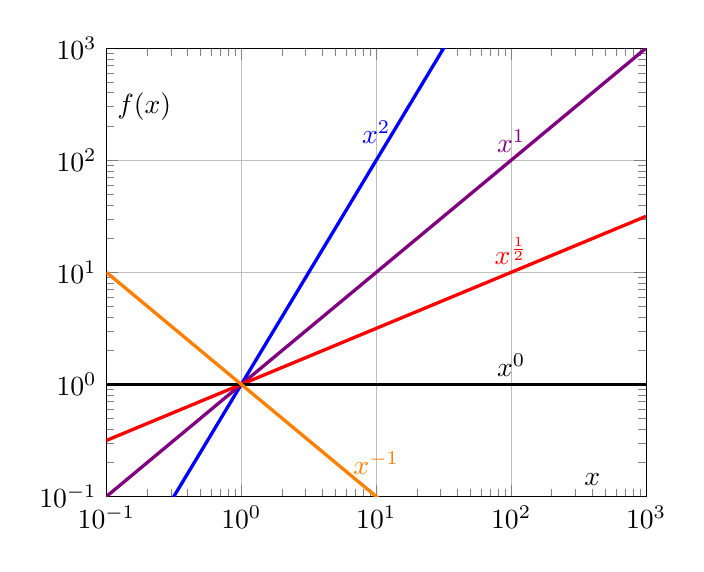
\begin{tikzpicture}
    % invisible boundbox
    \draw[draw=none](-1,-0.6) rectangle (+7.2,+5.9);
\begin{axis}[
    %title={Potenzfunktionen $x^n$, logarithmische Skalen},% außerhalb der boundbox
    xmode=log, ymode=log,% normal|linear|log
    xmin = 1e-1, xmax = 1e3,
    ymin = 1e-1, ymax = 1e3,
    domain = 1e-1:1e3,
    samples=41,
    %xtick distance=1,
    %ytick distance=1,
    minor x tick num=9,
    minor y tick num=9,
    grid=major,
]
    \addplot+[mark=none,very thick, blue] {x^2}     node[pos=0.500,anchor=south,yshift=+2pt] {$x^2$};
    %\addplot+[mark=none,very thick, violet] {2*x}   node[pos=0.925,anchor=south,yshift=-1pt] {$2x^1$};
    \addplot+[mark=none,very thick, violet] {x}     node[pos=0.750,anchor=south,yshift=-1pt] {$x^1$};
    \addplot+[mark=none, very thick, red] {x^0.5}   node[pos=0.750,anchor=south,yshift=-1pt] {$x^{\frac{1}{2}}$};
    \addplot+[mark=none, very thick, black] {1}     node[pos=0.750,anchor=south,yshift=-1pt] {$x^{0}$};
    \addplot+[mark=none, very thick, orange] {x^-1} node[pos=0.500,anchor=south,yshift=+4pt] {$x^{-1}$};
    % axis labels inside plot
    \addplot[mark=none, very thick, black] coordinates {(4e+2+0,1e-1)} node[anchor=south] {$x$}; % xlabel
    \addplot[mark=none, very thick, black] coordinates {(1e-1,3e+2)} node[anchor=west] {$f(x)$}; % ylabel
\end{axis}
\end{tikzpicture}